\documentclass[a4paper]{article}
\usepackage[OT1]{fontenc}
\usepackage{Sweave}
\begin{document}

\title{FunciSNP: Functional Identification of SNPs with\\Phenotype by 
Coincidence with Chromatin Biofeatures\\Vignette}
\author{Simon G. Coetzee and Houtan Noushmehr\\\\Norris Cancer Center\\Keck 
School of Medicine\\University of Southern California\\Los Angeles, USA.\\\\
and\\\\Faculdade de Medicina de Ribeir\^{a}o Preto\\Departmento de 
Gen\'{e}tica\\Universidade de S\^{a}o Paulo\\Ribeir\^{a}o Preto, S\^{a}o Paulo, 
Brasil}

\maketitle
\section*{Introduction}
%include intro text

\section*{Load FunciSNP+other useful libraries}
\begin{Schunk}
\begin{Sinput}
> #When package is offically posted in Bioconductor, uncomment next 2 lines.
> #source("http://bioconductor.org/biocLite.R")
> #biocLite("FunciSNP");
> ## Following two packages and options() are not required to run 'FunciSNP' but 
> #will enhance the analysis experience.
> #library(setwidth); ## Automatically set the value of options("width") when the 
> #terminal emulator is resized
> #library(colorout); ## colorize R output on terminal emulators
> options(width=80);
> ##FunciSNP library and other related libraries needed.
> library("org.Hs.eg.db");
> library("gplots");
> library("gtools");
> library("ggplot2");
> library("matlab");
> library(FunciSNP);
> package.version("FunciSNP");
\end{Sinput}
\begin{Soutput}
[1] "0.1.7"
\end{Soutput}
\end{Schunk}

\section*{Identify Func-y-SNP using published GWAS SNPs and publicly available 
biological features (ENCODE ChIPseq peaks)}
\subsection*{FunciSNP()}
This is the main funtion of FunciSNP. It will identify correlated SNPs which are
 in linkage disequilibrium (LD) to a known disease associated tagSNP. It will 
also determine if the correlated SNP in LD to the tagSNP overlaps a genomic 
biological feature. Correlated SNPs are directly imported from the current 
public release of the 1000 genomes database. 1000 genomes ftp servers available 
for the 1000 genomes public data: 1) National Center for Biotechnology 
Information (NCBI) ftp://ftp-trace.ncbi.nih.gov/1000genomes/; 2) European 
Bioinformatics Institute (EBI) ftp://ftp.1000genomes.ebi.ac.uk/vol1/.

Correlated SNPs in LD to a tagSNP and overlapping genomic biological features 
are known as putative functional SNPs (also defined as 'Func-y-SNP' elsewhere in
 the package.).

As an example, we collected SNPs identified by GWAS for Glioblastoma multiforme 
(GBM). In this example, GBM includes lower grade glioma, thus we label all 
objects with 'glioma'.
\begin{Schunk}
\begin{Sinput}
> ## Full path to the example GWAS SNP regions file for Glioblastoma 
> #  (collected from SNPedia on Jan 2012)
> glioma.snp <- file.path(system.file('data', package='FunciSNP'), 
+ dir(system.file('data',package='FunciSNP'), pattern='.snp$'));
> glioma.snp;
\end{Sinput}
\begin{Soutput}
[1] "/home/houtan/R/x86_64-pc-linux-gnu-library/2.14/FunciSNP/data/glioma.snp"
\end{Soutput}
\begin{Sinput}
> ## Full path to the example biological features BED files 
> #  derived from the ENCODE project for Glioblastoma U-87 cell lines.
> glioma.bio <- system.file('extdata',package='FunciSNP');
> glioma.bio;
\end{Sinput}
\begin{Soutput}
[1] "/home/houtan/R/x86_64-pc-linux-gnu-library/2.14/FunciSNP/extdata"
\end{Soutput}
\begin{Sinput}
> ## FunciSNP analysis, extracts correlated SNPs from the 
> #  1000 genomes db ("ncbi" or "ebi") and finds overlaps between 
> #  correlated SNP and biological features and then 
> #  calculates LD (Rsquare, Dprime, distance, p-value).
> glioma <- FunciSNP(snp.regions.file=glioma.snp, bio.features.loc = glioma.bio, 
+ bio.features.TSS=FALSE);
\end{Sinput}
\begin{Soutput}
Func-y-SNPs identified!!
Annotation will begin
~~
Adding lincRNA ... done
Adding gene annotations

Adding symbol ... done
Adding refseq ... done
prepare output ... done

Adding genomic annotations ... done

Now do the FunciStuff!
\end{Soutput}
\begin{Sinput}
> glioma;
\end{Sinput}
\begin{Soutput}
TagSNP List with  9  Tag SNPs and 
 969 nearby,  potentially correlated SNPs, that overlap at least one biofeature 
$`R squared: 0.1`
             Total R.squared.cuff.0.1 Percent
tagSNPs          7                  5   71.43
1kSNPs         969                 79    8.15
bio.features     3                  3  100.00

$`R squared: 0.5`
             Total R.squared.cuff.0.5 Percent
tagSNPs          7                  3   42.86
1kSNPs         969                 44    4.54
bio.features     2                  2  100.00

$`R squared: 0.9`
             Total R.squared.cuff.0.9 Percent
tagSNPs          7                  1   14.29
1kSNPs         969                 15    1.55
bio.features     2                  2  100.00
\end{Soutput}
\begin{Sinput}
> summary(glioma);
\end{Sinput}
\begin{Soutput}
TagSNP List with  9  Tag SNPs and 
 969 nearby,  potentially correlated SNPs, that overlap at least one biofeature 
Number of potentially correlated SNPs 
overlapping at least x biofeatures, per Tag SNP at an R squared of
$`R squared: 0.1 in 6 Tag SNPs with a total of `
                        bio.1 bio.2 bio.3 bio.4
rs11979158                  4     1     0     0
rs2252586                   1     0     0     0
rs4977756                   3     0     0     0
rs498872                   12     8     2     2
rs6010620                  59    53     9     9
TOTAL # CORRELATED SNPS    79    62    11    11

$`R squared: 0.5 in 4 Tag SNPs with a total of `
                        bio.1 bio.2 bio.3 bio.4
rs4977756                   2     0     0     0
rs498872                    2     2     0     0
rs6010620                  40    39     2     2
TOTAL # CORRELATED SNPS    44    41     2     2

$`R squared: 0.9 in 2 Tag SNPs with a total of `
                        bio.1 bio.2
rs6010620                  15    12
TOTAL # CORRELATED SNPS    15    12
\end{Soutput}
\begin{Sinput}
> ## The glioma example set can also be called by the following line if you don't 
> #want to redo the initial analysis. 
> data(glioma);
> glioma;
\end{Sinput}
\begin{Soutput}
TagSNP List with  9  Tag SNPs and 
 969 nearby,  potentially correlated SNPs, that overlap at least one biofeature 
$`R squared: 0.1`
             Total R.squared.cuff.0.1 Percent
tagSNPs          7                  5   71.43
1kSNPs         969                 79    8.15
bio.features     3                  3  100.00

$`R squared: 0.5`
             Total R.squared.cuff.0.5 Percent
tagSNPs          7                  3   42.86
1kSNPs         969                 44    4.54
bio.features     2                  2  100.00

$`R squared: 0.9`
             Total R.squared.cuff.0.9 Percent
tagSNPs          7                  1   14.29
1kSNPs         969                 15    1.55
bio.features     2                  2  100.00
\end{Soutput}
\begin{Sinput}
> summary(glioma);
\end{Sinput}
\begin{Soutput}
TagSNP List with  9  Tag SNPs and 
 969 nearby,  potentially correlated SNPs, that overlap at least one biofeature 
Number of potentially correlated SNPs 
overlapping at least x biofeatures, per Tag SNP at an R squared of
$`R squared: 0.1 in 6 Tag SNPs with a total of `
                        bio.1 bio.2 bio.3 bio.4
rs11979158                  4     1     0     0
rs2252586                   1     0     0     0
rs4977756                   3     0     0     0
rs498872                   12     8     2     2
rs6010620                  59    53     9     9
TOTAL # CORRELATED SNPS    79    62    11    11

$`R squared: 0.5 in 4 Tag SNPs with a total of `
                        bio.1 bio.2 bio.3 bio.4
rs4977756                   2     0     0     0
rs498872                    2     2     0     0
rs6010620                  40    39     2     2
TOTAL # CORRELATED SNPS    44    41     2     2

$`R squared: 0.9 in 2 Tag SNPs with a total of `
                        bio.1 bio.2
rs6010620                  15    12
TOTAL # CORRELATED SNPS    15    12
\end{Soutput}
\end{Schunk}

\subsection*{FunciSNPAnnotateSummary()}
All known genomic features (exon, intron, 5'UTR, 3'UTR, promoter, lincRNA or in 
gene desert (intergentic)) are used to annotate the newly identified Func-y-SNP.
 Information described in this data.frame is used for all summary plots, table, 
 and bed file generations.
\begin{Schunk}
\begin{Sinput}
> glioma.anno <- FunciSNPAnnotateSummary(glioma);
> summary(glioma.anno);
\end{Sinput}
\begin{Soutput}
  chromosome        bio.feature.start  bio.feature.end   
 Length:1800        Min.   :1.20e+06   Min.   :1.20e+06  
 Class :character   1st Qu.:6.23e+07   1st Qu.:6.23e+07  
 Mode  :character   Median :6.23e+07   Median :6.23e+07  
                    Mean   :6.96e+07   Mean   :6.96e+07  
                    3rd Qu.:6.24e+07   3rd Qu.:6.24e+07  
                    Max.   :1.31e+08   Max.   :1.31e+08  
                                                         
             bio.feature            corr.snp.id   corr.snp.position 
 knownGene.TSS.hg19: 695   chr11:118442863:   4   Min.   :1.20e+06  
 TFBS_Nrsf_U87     :  26   chr11:118443036:   4   1st Qu.:6.23e+07  
 TFBS_Pol2_U87     :1079   chr11:118443046:   4   Median :6.23e+07  
                           chr11:118478342:   4   Mean   :6.96e+07  
                           chr20:62289690 :   4   3rd Qu.:6.24e+07  
                           chr20:62289873 :   4   Max.   :1.31e+08  
                           (Other)        :1776                     
      tag.snp.id   tag.snp.position      D.prime           R.squared       
 rs11979158: 143   Min.   :1.29e+06   Min.   :7.84e-04   Min.   :9.52e-08  
 rs2252586 :  17   1st Qu.:6.23e+07   1st Qu.:9.13e-01   1st Qu.:1.17e-03  
 rs2736100 :  96   Median :6.23e+07   Median :1.00e+00   Median :5.45e-03  
 rs4295627 :  37   Mean   :6.96e+07   Mean   :8.87e-01   Mean   :1.40e-01  
 rs4977756 :  25   3rd Qu.:6.23e+07   3rd Qu.:1.00e+00   3rd Qu.:8.70e-02  
 rs498872  : 332   Max.   :1.31e+08   Max.   :1.00e+00   Max.   :1.00e+00  
 rs6010620 :1150                      NA's   :1.12e+03   NA's   :1.12e+03  
    p.value          distance.from.tag population.count population
 Min.   :2.11e-163   Min.   :-100000   Min.   :286      ASN:837   
 1st Qu.: 1.00e+00   1st Qu.:   -731   1st Qu.:286      EUR:963   
 Median : 1.00e+00   Median :  15546   Median :379                
 Mean   : 8.21e-01   Mean   :   8971   Mean   :336                
 3rd Qu.: 1.00e+00   3rd Qu.:  27362   3rd Qu.:379                
 Max.   : 1.00e+00   Max.   :  95365   Max.   :379                
                                                                  
      nearest.lincRNA.ID nearest.lincRNA.distancetoFeature
 TCONS_00010241:  96     Min.   :-375171                  
 TCONS_00013806: 160     1st Qu.:-160171                  
 TCONS_00014564:  37     Median :  57264                  
 TCONS_00015797:  25     Mean   : -21083                  
 TCONS_00020001: 332     3rd Qu.:  71934                  
 TCONS_00027984:  52     Max.   : 246019                  
 TCONS_00028269:1098                                      
 nearest.lincRNA.coverage    nearest.TSS.GeneSymbol
 downstream:1105          TNFRSF6B      :610       
 inside    :  21          PHLDB1        :172       
 upstream  : 674          ZGPAT         :136       
                          EGFR          : 77       
                          RTEL1;TNFRSF6B: 74       
                          (Other)       :391       
                          NA's          :340       
   
      nearest.TSS.ensembl nearest.TSS.coverage nearest.TSS.distancetoFeature
 ENSG00000243509:610      downstream:240       Min.   :-93691               
 ENSG00000019144:172      inside    :664       1st Qu.: -3652               
 ENSG00000197114:136      upstream  :896       Median :    13               
 ENSG00000229299:118                           Mean   :  2926               
 ENSG00000224057: 82                           3rd Qu.:  2781               
 ENSG00000146648: 77                           Max.   : 80077               
 (Other)        :605                                                        
 Promoter    utr5       Exon      Intron     utr3      Intergenic
 NO :1495   NO :1725   NO :1629   NO :811   NO :1508   NO :1670  
 YES: 305   YES:  75   YES: 171   YES:989   YES: 292   YES: 130  
\end{Soutput}
\begin{Sinput}
> dim(glioma.anno)
\end{Sinput}
\begin{Soutput}
[1] 1800   28
\end{Soutput}
\begin{Sinput}
> head(glioma.anno)
\end{Sinput}
\begin{Soutput}
                                                chromosome bio.feature.start
rs11979158:EUR.chr7:55085731.knownGene.TSS.hg19          7          55085725
rs11979158:EUR.chr7:55085897.knownGene.TSS.hg19          7          55085725
rs11979158:EUR.chr7:55086373.knownGene.TSS.hg19          7          55085725
rs11979158:EUR.chr7:55086373.TFBS_Pol2_U87               7          55086315
rs11979158:EUR.chr7:55086393.knownGene.TSS.hg19          7          55085725
rs11979158:EUR.chr7:55086393.TFBS_Pol2_U87               7          55086315
                                                bio.feature.end
rs11979158:EUR.chr7:55085731.knownGene.TSS.hg19        55086824
rs11979158:EUR.chr7:55085897.knownGene.TSS.hg19        55086824
rs11979158:EUR.chr7:55086373.knownGene.TSS.hg19        55086824
rs11979158:EUR.chr7:55086373.TFBS_Pol2_U87             55087150
rs11979158:EUR.chr7:55086393.knownGene.TSS.hg19        55086824
rs11979158:EUR.chr7:55086393.TFBS_Pol2_U87             55087150
                                                       bio.feature
rs11979158:EUR.chr7:55085731.knownGene.TSS.hg19 knownGene.TSS.hg19
rs11979158:EUR.chr7:55085897.knownGene.TSS.hg19 knownGene.TSS.hg19
rs11979158:EUR.chr7:55086373.knownGene.TSS.hg19 knownGene.TSS.hg19
rs11979158:EUR.chr7:55086373.TFBS_Pol2_U87           TFBS_Pol2_U87
rs11979158:EUR.chr7:55086393.knownGene.TSS.hg19 knownGene.TSS.hg19
rs11979158:EUR.chr7:55086393.TFBS_Pol2_U87           TFBS_Pol2_U87
                                                  corr.snp.id corr.snp.position
rs11979158:EUR.chr7:55085731.knownGene.TSS.hg19 chr7:55085731          55085731
rs11979158:EUR.chr7:55085897.knownGene.TSS.hg19 chr7:55085897          55085897
rs11979158:EUR.chr7:55086373.knownGene.TSS.hg19 chr7:55086373          55086373
rs11979158:EUR.chr7:55086373.TFBS_Pol2_U87      chr7:55086373          55086373
rs11979158:EUR.chr7:55086393.knownGene.TSS.hg19 chr7:55086393          55086393
rs11979158:EUR.chr7:55086393.TFBS_Pol2_U87      chr7:55086393          55086393
                                                tag.snp.id tag.snp.position
rs11979158:EUR.chr7:55085731.knownGene.TSS.hg19 rs11979158         55159349
rs11979158:EUR.chr7:55085897.knownGene.TSS.hg19 rs11979158         55159349
rs11979158:EUR.chr7:55086373.knownGene.TSS.hg19 rs11979158         55159349
rs11979158:EUR.chr7:55086373.TFBS_Pol2_U87      rs11979158         55159349
rs11979158:EUR.chr7:55086393.knownGene.TSS.hg19 rs11979158         55159349
rs11979158:EUR.chr7:55086393.TFBS_Pol2_U87      rs11979158         55159349
                                                D.prime R.squared p.value
rs11979158:EUR.chr7:55085731.knownGene.TSS.hg19      NA        NA       1
rs11979158:EUR.chr7:55085897.knownGene.TSS.hg19      NA        NA       1
rs11979158:EUR.chr7:55086373.knownGene.TSS.hg19      NA        NA       1
rs11979158:EUR.chr7:55086373.TFBS_Pol2_U87           NA        NA       1
rs11979158:EUR.chr7:55086393.knownGene.TSS.hg19      NA        NA       1
rs11979158:EUR.chr7:55086393.TFBS_Pol2_U87           NA        NA       1
                                                distance.from.tag
rs11979158:EUR.chr7:55085731.knownGene.TSS.hg19            -73618
rs11979158:EUR.chr7:55085897.knownGene.TSS.hg19            -73452
rs11979158:EUR.chr7:55086373.knownGene.TSS.hg19            -72976
rs11979158:EUR.chr7:55086373.TFBS_Pol2_U87                 -72976
rs11979158:EUR.chr7:55086393.knownGene.TSS.hg19            -72956
rs11979158:EUR.chr7:55086393.TFBS_Pol2_U87                 -72956
                                                population.count population
rs11979158:EUR.chr7:55085731.knownGene.TSS.hg19              379        EUR
rs11979158:EUR.chr7:55085897.knownGene.TSS.hg19              379        EUR
rs11979158:EUR.chr7:55086373.knownGene.TSS.hg19              379        EUR
rs11979158:EUR.chr7:55086373.TFBS_Pol2_U87                   379        EUR
rs11979158:EUR.chr7:55086393.knownGene.TSS.hg19              379        EUR
rs11979158:EUR.chr7:55086393.TFBS_Pol2_U87                   379        EUR
                                                nearest.lincRNA.ID
rs11979158:EUR.chr7:55085731.knownGene.TSS.hg19     TCONS_00013806
rs11979158:EUR.chr7:55085897.knownGene.TSS.hg19     TCONS_00013806
rs11979158:EUR.chr7:55086373.knownGene.TSS.hg19     TCONS_00013806
rs11979158:EUR.chr7:55086373.TFBS_Pol2_U87          TCONS_00013806
rs11979158:EUR.chr7:55086393.knownGene.TSS.hg19     TCONS_00013806
rs11979158:EUR.chr7:55086393.TFBS_Pol2_U87          TCONS_00013806
                                                nearest.lincRNA.distancetoFeature
rs11979158:EUR.chr7:55085731.knownGene.TSS.hg19                           -206188
rs11979158:EUR.chr7:55085897.knownGene.TSS.hg19                           -206354
rs11979158:EUR.chr7:55086373.knownGene.TSS.hg19                           -206830
rs11979158:EUR.chr7:55086373.TFBS_Pol2_U87                                -206830
rs11979158:EUR.chr7:55086393.knownGene.TSS.hg19                           -206850
rs11979158:EUR.chr7:55086393.TFBS_Pol2_U87                                -206850
                                                nearest.lincRNA.coverage
rs11979158:EUR.chr7:55085731.knownGene.TSS.hg19                 upstream
rs11979158:EUR.chr7:55085897.knownGene.TSS.hg19                 upstream
rs11979158:EUR.chr7:55086373.knownGene.TSS.hg19                 upstream
rs11979158:EUR.chr7:55086373.TFBS_Pol2_U87                      upstream
rs11979158:EUR.chr7:55086393.knownGene.TSS.hg19                 upstream
rs11979158:EUR.chr7:55086393.TFBS_Pol2_U87                      upstream
                                                nearest.TSS.GeneSymbol
rs11979158:EUR.chr7:55085731.knownGene.TSS.hg19                   EGFR
rs11979158:EUR.chr7:55085897.knownGene.TSS.hg19                   EGFR
rs11979158:EUR.chr7:55086373.knownGene.TSS.hg19                   EGFR
rs11979158:EUR.chr7:55086373.TFBS_Pol2_U87                        EGFR
rs11979158:EUR.chr7:55086393.knownGene.TSS.hg19                   EGFR
rs11979158:EUR.chr7:55086393.TFBS_Pol2_U87                        EGFR

                                                nearest.TSS.ensembl
rs11979158:EUR.chr7:55085731.knownGene.TSS.hg19     ENSG00000146648
rs11979158:EUR.chr7:55085897.knownGene.TSS.hg19     ENSG00000146648
rs11979158:EUR.chr7:55086373.knownGene.TSS.hg19     ENSG00000146648
rs11979158:EUR.chr7:55086373.TFBS_Pol2_U87          ENSG00000146648
rs11979158:EUR.chr7:55086393.knownGene.TSS.hg19     ENSG00000146648
rs11979158:EUR.chr7:55086393.TFBS_Pol2_U87          ENSG00000146648
                                                nearest.TSS.coverage
rs11979158:EUR.chr7:55085731.knownGene.TSS.hg19             upstream
rs11979158:EUR.chr7:55085897.knownGene.TSS.hg19             upstream
rs11979158:EUR.chr7:55086373.knownGene.TSS.hg19             upstream
rs11979158:EUR.chr7:55086373.TFBS_Pol2_U87                  upstream
rs11979158:EUR.chr7:55086393.knownGene.TSS.hg19             upstream
rs11979158:EUR.chr7:55086393.TFBS_Pol2_U87                  upstream
                                                nearest.TSS.distancetoFeature
rs11979158:EUR.chr7:55085731.knownGene.TSS.hg19                          -983
rs11979158:EUR.chr7:55085897.knownGene.TSS.hg19                          -817
rs11979158:EUR.chr7:55086373.knownGene.TSS.hg19                          -341
rs11979158:EUR.chr7:55086373.TFBS_Pol2_U87                               -341
rs11979158:EUR.chr7:55086393.knownGene.TSS.hg19                          -321
rs11979158:EUR.chr7:55086393.TFBS_Pol2_U87                               -321
                                                Promoter utr5 Exon Intron utr3
rs11979158:EUR.chr7:55085731.knownGene.TSS.hg19      YES   NO   NO     NO   NO
rs11979158:EUR.chr7:55085897.knownGene.TSS.hg19      YES   NO   NO     NO   NO
rs11979158:EUR.chr7:55086373.knownGene.TSS.hg19      YES   NO   NO     NO   NO
rs11979158:EUR.chr7:55086373.TFBS_Pol2_U87           YES   NO   NO     NO   NO
rs11979158:EUR.chr7:55086393.knownGene.TSS.hg19      YES   NO   NO     NO   NO
rs11979158:EUR.chr7:55086393.TFBS_Pol2_U87           YES   NO   NO     NO   NO
                                                Intergenic
rs11979158:EUR.chr7:55085731.knownGene.TSS.hg19         NO
rs11979158:EUR.chr7:55085897.knownGene.TSS.hg19         NO
rs11979158:EUR.chr7:55086373.knownGene.TSS.hg19         NO
rs11979158:EUR.chr7:55086373.TFBS_Pol2_U87              NO
rs11979158:EUR.chr7:55086393.knownGene.TSS.hg19         NO
rs11979158:EUR.chr7:55086393.TFBS_Pol2_U87              NO
\end{Soutput}
\begin{Sinput}
> names(glioma.anno)
\end{Sinput}
\begin{Soutput}
 [1] "chromosome"                        "bio.feature.start"                
 [3] "bio.feature.end"                   "bio.feature"                      
 [5] "corr.snp.id"                       "corr.snp.position"                
 [7] "tag.snp.id"                        "tag.snp.position"                 
 [9] "D.prime"                           "R.squared"                        
[11] "p.value"                           "distance.from.tag"                
[13] "population.count"                  "population"                       
[15] "nearest.lincRNA.ID"                "nearest.lincRNA.distancetoFeature"
[17] "nearest.lincRNA.coverage"          "nearest.TSS.GeneSymbol"           
[19] "nearest.TSS.refseq"                "nearest.TSS.ensembl"              
[21] "nearest.TSS.coverage"              "nearest.TSS.distancetoFeature"    
[23] "Promoter"                          "utr5"                             
[25] "Exon"                              "Intron"                           
[27] "utr3"                              "Intergenic"                       
\end{Soutput}
\end{Schunk}
\subsection*{FunciSNPtable()}
Using a specified Rsquare value (0-1) to subset the data, a table is generated 
which summarizes the total number of Func-y-SNPs, associated tagSNPs, and number
 of overlapping biofeatures. This will provide user a first look at the total 
 number of available Func-y-SNP at a particular Rsquare cutoff.  If geneSum is 
 set to TRUE, a list of gene names is reported instead.
\begin{Schunk}
\begin{Sinput}
> FunciSNPtable(glioma.anno, rsq=0.5);
\end{Sinput}
\begin{Soutput}
             Total R.squared.cuff.0.5 Percent
tagSNPs          7                  3   42.86
1kSNPs         969                 44    4.54
bio.features     2                  2  100.00
\end{Soutput}
\begin{Sinput}
> FunciSNPtable(glioma.anno, rsq=0.5, geneSum=T);
\end{Sinput}
\begin{Soutput}
      Gene_Names
1         CDKN2B
2          LIME1
3         PHLDB1
4       SLC2A4RG
5       TNFRSF6B
6           TREH
7          ZGPAT
8 RTEL1;TNFRSF6B
\end{Soutput}
\end{Schunk}
\subsection*{FunciSNPsummaryOverlaps()}
\begin{Schunk}
\begin{Sinput}
> FunciSNPsummaryOverlaps(glioma.anno)
\end{Sinput}
\begin{Soutput}
                        bio.1 bio.2 bio.3 bio.4
rs11979158                 55     2     0     0
rs2252586                   5     0     0     0
rs2736100                  41     0     0     0
rs4295627                  13     0     0     0
rs4977756                  12     0     0     0
rs498872                   82    18     2     2
rs6010620                 294   119    17    17
TOTAL # CORRELATED SNPS   502   139    19    19
\end{Soutput}
\begin{Sinput}
> FunciSNPsummaryOverlaps(glioma.anno, rsq=0.5)
\end{Sinput}
\begin{Soutput}
                        bio.1 bio.2 bio.3 bio.4
rs4977756                   2     0     0     0
rs498872                    2     2     0     0
rs6010620                  40    39     2     2
TOTAL # CORRELATED SNPS    44    41     2     2
\end{Soutput}
\end{Schunk}
\subsection*{FunciSNPidsFromSummary()}
\begin{Schunk}
\begin{Sinput}
> FunciSNPidsFromSummary(glioma.anno, tagsnpid="rs6010620", num.features=3, 
+ rsq=0.5)
\end{Sinput}
\begin{Soutput}
                                           chromosome bio.feature.start
rs6010620:ASN.rs1291209.knownGene.TSS.hg19         20          62329895
rs6010620:ASN.rs1291209.TFBS_Pol2_U87              20          62326155
rs6010620:EUR.rs1291209.knownGene.TSS.hg19         20          62329895
rs6010620:EUR.rs1291209.TFBS_Pol2_U87              20          62326155
rs6010620:ASN.rs1295810.knownGene.TSS.hg19         20          62329895
rs6010620:ASN.rs1295810.TFBS_Pol2_U87              20          62326155
rs6010620:EUR.rs1295810.knownGene.TSS.hg19         20          62329895
rs6010620:EUR.rs1295810.TFBS_Pol2_U87              20          62326155
                                           bio.feature.end        bio.feature
rs6010620:ASN.rs1291209.knownGene.TSS.hg19        62330994 knownGene.TSS.hg19
rs6010620:ASN.rs1291209.TFBS_Pol2_U87             62337392      TFBS_Pol2_U87
rs6010620:EUR.rs1291209.knownGene.TSS.hg19        62330994 knownGene.TSS.hg19
rs6010620:EUR.rs1291209.TFBS_Pol2_U87             62337392      TFBS_Pol2_U87
rs6010620:ASN.rs1295810.knownGene.TSS.hg19        62330994 knownGene.TSS.hg19
rs6010620:ASN.rs1295810.TFBS_Pol2_U87             62337392      TFBS_Pol2_U87
rs6010620:EUR.rs1295810.knownGene.TSS.hg19        62330994 knownGene.TSS.hg19
rs6010620:EUR.rs1295810.TFBS_Pol2_U87             62337392      TFBS_Pol2_U87
                                           corr.snp.id corr.snp.position
rs6010620:ASN.rs1291209.knownGene.TSS.hg19   rs1291209          62330439
rs6010620:ASN.rs1291209.TFBS_Pol2_U87        rs1291209          62330439
rs6010620:EUR.rs1291209.knownGene.TSS.hg19   rs1291209          62330439
rs6010620:EUR.rs1291209.TFBS_Pol2_U87        rs1291209          62330439
rs6010620:ASN.rs1295810.knownGene.TSS.hg19   rs1295810          62330484
rs6010620:ASN.rs1295810.TFBS_Pol2_U87        rs1295810          62330484
rs6010620:EUR.rs1295810.knownGene.TSS.hg19   rs1295810          62330484
rs6010620:EUR.rs1295810.TFBS_Pol2_U87        rs1295810          62330484
                                           tag.snp.id tag.snp.position D.prime
rs6010620:ASN.rs1291209.knownGene.TSS.hg19  rs6010620         62309839  0.9032
rs6010620:ASN.rs1291209.TFBS_Pol2_U87       rs6010620         62309839  0.9032
rs6010620:EUR.rs1291209.knownGene.TSS.hg19  rs6010620         62309839  0.9204
rs6010620:EUR.rs1291209.TFBS_Pol2_U87       rs6010620         62309839  0.9204
rs6010620:ASN.rs1295810.knownGene.TSS.hg19  rs6010620         62309839  0.9032
rs6010620:ASN.rs1295810.TFBS_Pol2_U87       rs6010620         62309839  0.9032
rs6010620:EUR.rs1295810.knownGene.TSS.hg19  rs6010620         62309839  0.9204
rs6010620:EUR.rs1295810.TFBS_Pol2_U87       rs6010620         62309839  0.9204
                                           R.squared    p.value
rs6010620:ASN.rs1291209.knownGene.TSS.hg19    0.5696  2.786e-75
rs6010620:ASN.rs1291209.TFBS_Pol2_U87         0.5696  2.786e-75
rs6010620:EUR.rs1291209.knownGene.TSS.hg19    0.8092 1.555e-127
rs6010620:EUR.rs1291209.TFBS_Pol2_U87         0.8092 1.555e-127
rs6010620:ASN.rs1295810.knownGene.TSS.hg19    0.5696  2.786e-75
rs6010620:ASN.rs1295810.TFBS_Pol2_U87         0.5696  2.786e-75
rs6010620:EUR.rs1295810.knownGene.TSS.hg19    0.8092 1.555e-127
rs6010620:EUR.rs1295810.TFBS_Pol2_U87         0.8092 1.555e-127
                                           distance.from.tag population.count
rs6010620:ASN.rs1291209.knownGene.TSS.hg19             20600              286
rs6010620:ASN.rs1291209.TFBS_Pol2_U87                  20600              286
rs6010620:EUR.rs1291209.knownGene.TSS.hg19             20600              379
rs6010620:EUR.rs1291209.TFBS_Pol2_U87                  20600              379
rs6010620:ASN.rs1295810.knownGene.TSS.hg19             20645              286
rs6010620:ASN.rs1295810.TFBS_Pol2_U87                  20645              286
rs6010620:EUR.rs1295810.knownGene.TSS.hg19             20645              379
rs6010620:EUR.rs1295810.TFBS_Pol2_U87                  20645              379
                                           population nearest.lincRNA.ID
rs6010620:ASN.rs1291209.knownGene.TSS.hg19        ASN     TCONS_00028269
rs6010620:ASN.rs1291209.TFBS_Pol2_U87             ASN     TCONS_00028269
rs6010620:EUR.rs1291209.knownGene.TSS.hg19        EUR     TCONS_00028269
rs6010620:EUR.rs1291209.TFBS_Pol2_U87             EUR     TCONS_00028269
rs6010620:ASN.rs1295810.knownGene.TSS.hg19        ASN     TCONS_00028269
rs6010620:ASN.rs1295810.TFBS_Pol2_U87             ASN     TCONS_00028269
rs6010620:EUR.rs1295810.knownGene.TSS.hg19        EUR     TCONS_00028269
rs6010620:EUR.rs1295810.TFBS_Pol2_U87             EUR     TCONS_00028269
                                           nearest.lincRNA.distancetoFeature
rs6010620:ASN.rs1291209.knownGene.TSS.hg19                             71755
rs6010620:ASN.rs1291209.TFBS_Pol2_U87                                  71755
rs6010620:EUR.rs1291209.knownGene.TSS.hg19                             71755
rs6010620:EUR.rs1291209.TFBS_Pol2_U87                                  71755
rs6010620:ASN.rs1295810.knownGene.TSS.hg19                             71800
rs6010620:ASN.rs1295810.TFBS_Pol2_U87                                  71800
rs6010620:EUR.rs1295810.knownGene.TSS.hg19                             71800
rs6010620:EUR.rs1295810.TFBS_Pol2_U87                                  71800
                                           nearest.lincRNA.coverage
rs6010620:ASN.rs1291209.knownGene.TSS.hg19               downstream
rs6010620:ASN.rs1291209.TFBS_Pol2_U87                    downstream
rs6010620:EUR.rs1291209.knownGene.TSS.hg19               downstream
rs6010620:EUR.rs1291209.TFBS_Pol2_U87                    downstream
rs6010620:ASN.rs1295810.knownGene.TSS.hg19               downstream
rs6010620:ASN.rs1295810.TFBS_Pol2_U87                    downstream
rs6010620:EUR.rs1295810.knownGene.TSS.hg19               downstream
rs6010620:EUR.rs1295810.TFBS_Pol2_U87                    downstream
                                           nearest.TSS.GeneSymbol
rs6010620:ASN.rs1291209.knownGene.TSS.hg19               TNFRSF6B
rs6010620:ASN.rs1291209.TFBS_Pol2_U87                    TNFRSF6B
rs6010620:EUR.rs1291209.knownGene.TSS.hg19               TNFRSF6B
rs6010620:EUR.rs1291209.TFBS_Pol2_U87                    TNFRSF6B
rs6010620:ASN.rs1295810.knownGene.TSS.hg19               TNFRSF6B
rs6010620:ASN.rs1295810.TFBS_Pol2_U87                    TNFRSF6B
rs6010620:EUR.rs1295810.knownGene.TSS.hg19               TNFRSF6B
rs6010620:EUR.rs1295810.TFBS_Pol2_U87                    TNFRSF6B
                                            nearest.TSS.refseq
rs6010620:ASN.rs1291209.knownGene.TSS.hg19 NM_003823;NP_003814
rs6010620:ASN.rs1291209.TFBS_Pol2_U87      NM_003823;NP_003814
rs6010620:EUR.rs1291209.knownGene.TSS.hg19 NM_003823;NP_003814
rs6010620:EUR.rs1291209.TFBS_Pol2_U87      NM_003823;NP_003814
rs6010620:ASN.rs1295810.knownGene.TSS.hg19 NM_003823;NP_003814
rs6010620:ASN.rs1295810.TFBS_Pol2_U87      NM_003823;NP_003814
rs6010620:EUR.rs1295810.knownGene.TSS.hg19 NM_003823;NP_003814
rs6010620:EUR.rs1295810.TFBS_Pol2_U87      NM_003823;NP_003814
                                           nearest.TSS.ensembl
rs6010620:ASN.rs1291209.knownGene.TSS.hg19     ENSG00000243509
rs6010620:ASN.rs1291209.TFBS_Pol2_U87          ENSG00000243509
rs6010620:EUR.rs1291209.knownGene.TSS.hg19     ENSG00000243509
rs6010620:EUR.rs1291209.TFBS_Pol2_U87          ENSG00000243509
rs6010620:ASN.rs1295810.knownGene.TSS.hg19     ENSG00000243509
rs6010620:ASN.rs1295810.TFBS_Pol2_U87          ENSG00000243509
rs6010620:EUR.rs1295810.knownGene.TSS.hg19     ENSG00000243509
rs6010620:EUR.rs1295810.TFBS_Pol2_U87          ENSG00000243509
                                           nearest.TSS.coverage
rs6010620:ASN.rs1291209.knownGene.TSS.hg19           downstream
rs6010620:ASN.rs1291209.TFBS_Pol2_U87                downstream
rs6010620:EUR.rs1291209.knownGene.TSS.hg19           downstream
rs6010620:EUR.rs1291209.TFBS_Pol2_U87                downstream
rs6010620:ASN.rs1295810.knownGene.TSS.hg19           downstream
rs6010620:ASN.rs1295810.TFBS_Pol2_U87                downstream
rs6010620:EUR.rs1295810.knownGene.TSS.hg19           downstream
rs6010620:EUR.rs1295810.TFBS_Pol2_U87                downstream
                                           nearest.TSS.distancetoFeature
rs6010620:ASN.rs1291209.knownGene.TSS.hg19                          2418
rs6010620:ASN.rs1291209.TFBS_Pol2_U87                               2418
rs6010620:EUR.rs1291209.knownGene.TSS.hg19                          2418
rs6010620:EUR.rs1291209.TFBS_Pol2_U87                               2418
rs6010620:ASN.rs1295810.knownGene.TSS.hg19                          2463
rs6010620:ASN.rs1295810.TFBS_Pol2_U87                               2463
rs6010620:EUR.rs1295810.knownGene.TSS.hg19                          2463
rs6010620:EUR.rs1295810.TFBS_Pol2_U87                               2463
                                           Promoter utr5 Exon Intron utr3
rs6010620:ASN.rs1291209.knownGene.TSS.hg19       NO   NO   NO     NO  YES
rs6010620:ASN.rs1291209.TFBS_Pol2_U87            NO   NO   NO     NO  YES
rs6010620:EUR.rs1291209.knownGene.TSS.hg19       NO   NO   NO     NO  YES
rs6010620:EUR.rs1291209.TFBS_Pol2_U87            NO   NO   NO     NO  YES
rs6010620:ASN.rs1295810.knownGene.TSS.hg19       NO   NO   NO     NO  YES
rs6010620:ASN.rs1295810.TFBS_Pol2_U87            NO   NO   NO     NO  YES
rs6010620:EUR.rs1295810.knownGene.TSS.hg19       NO   NO   NO     NO  YES
rs6010620:EUR.rs1295810.TFBS_Pol2_U87            NO   NO   NO     NO  YES
                                           Intergenic
rs6010620:ASN.rs1291209.knownGene.TSS.hg19         NO
rs6010620:ASN.rs1291209.TFBS_Pol2_U87              NO
rs6010620:EUR.rs1291209.knownGene.TSS.hg19         NO
rs6010620:EUR.rs1291209.TFBS_Pol2_U87              NO
rs6010620:ASN.rs1295810.knownGene.TSS.hg19         NO
rs6010620:ASN.rs1295810.TFBS_Pol2_U87              NO
rs6010620:EUR.rs1295810.knownGene.TSS.hg19         NO
rs6010620:EUR.rs1295810.TFBS_Pol2_U87              NO
\end{Soutput}
\end{Schunk}

\subsection*{FunciSNPplot()}
FunciSNPplot is a function developed to plot various types of plots to summarize
 and assist end-user in making informed discoveries of FunciSNP results. Plots 
 can be stored in a folder for future reference.
\begin{Schunk}
\begin{Sinput}
> pdf("glioma_dist.pdf")
> FunciSNPplot(glioma.anno)
> dev.off()
\end{Sinput}
\begin{Soutput}
null device 
          1 
\end{Soutput}
\end{Schunk}
\begin{figure}[ht!]
\begin{center}
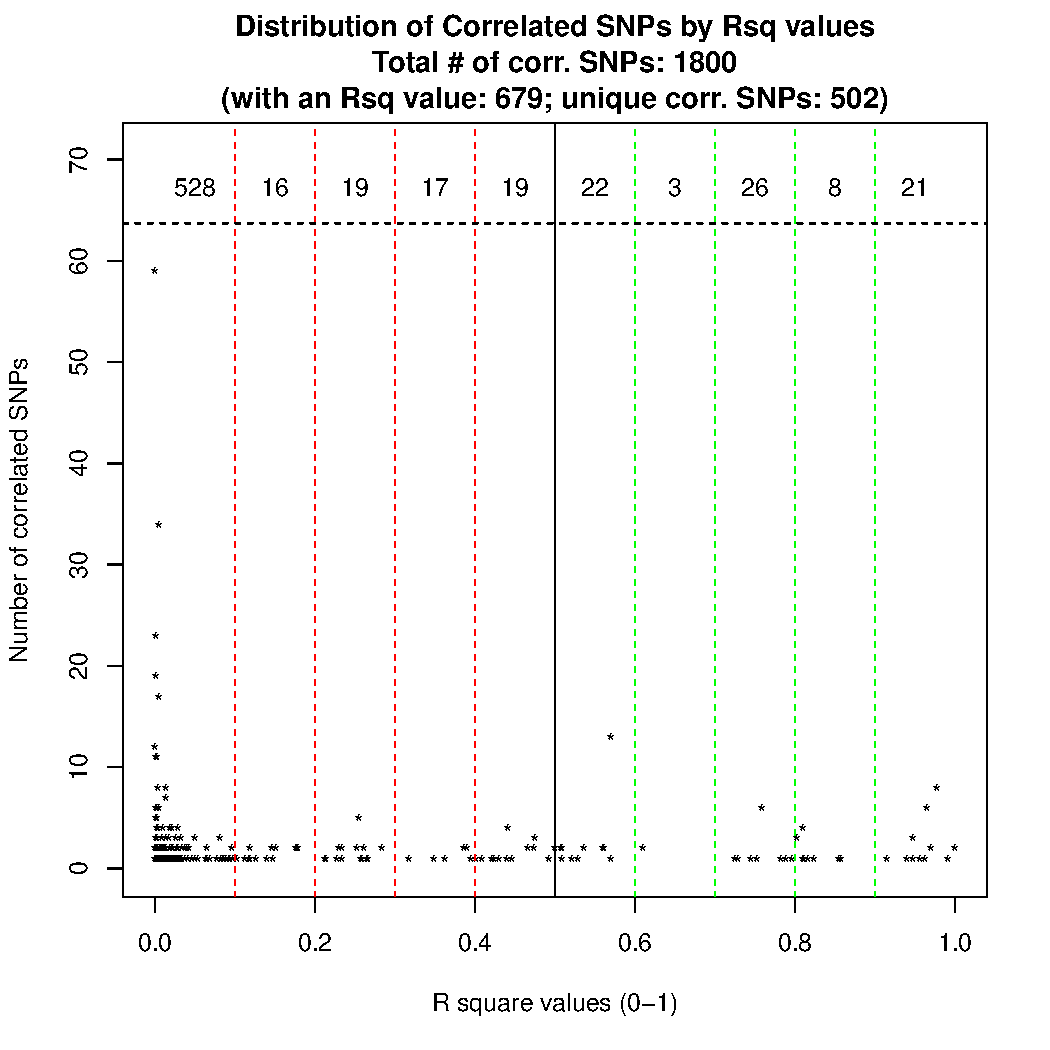
\includegraphics{glioma_dist.pdf}
\caption{\label{fig:glioma_dist.pdf} Distribution of Rsquare values of all 
Correlated SNPs}
{\footnotesize{}}
\end{center}
\end{figure}

\begin{Schunk}
\begin{Sinput}
> FunciSNPplot(glioma.anno, splitbysnp=T)
> ggsave("glioma_dist_bysnp.pdf")
\end{Sinput}
\end{Schunk}
\begin{figure}[ht!]
\begin{center}
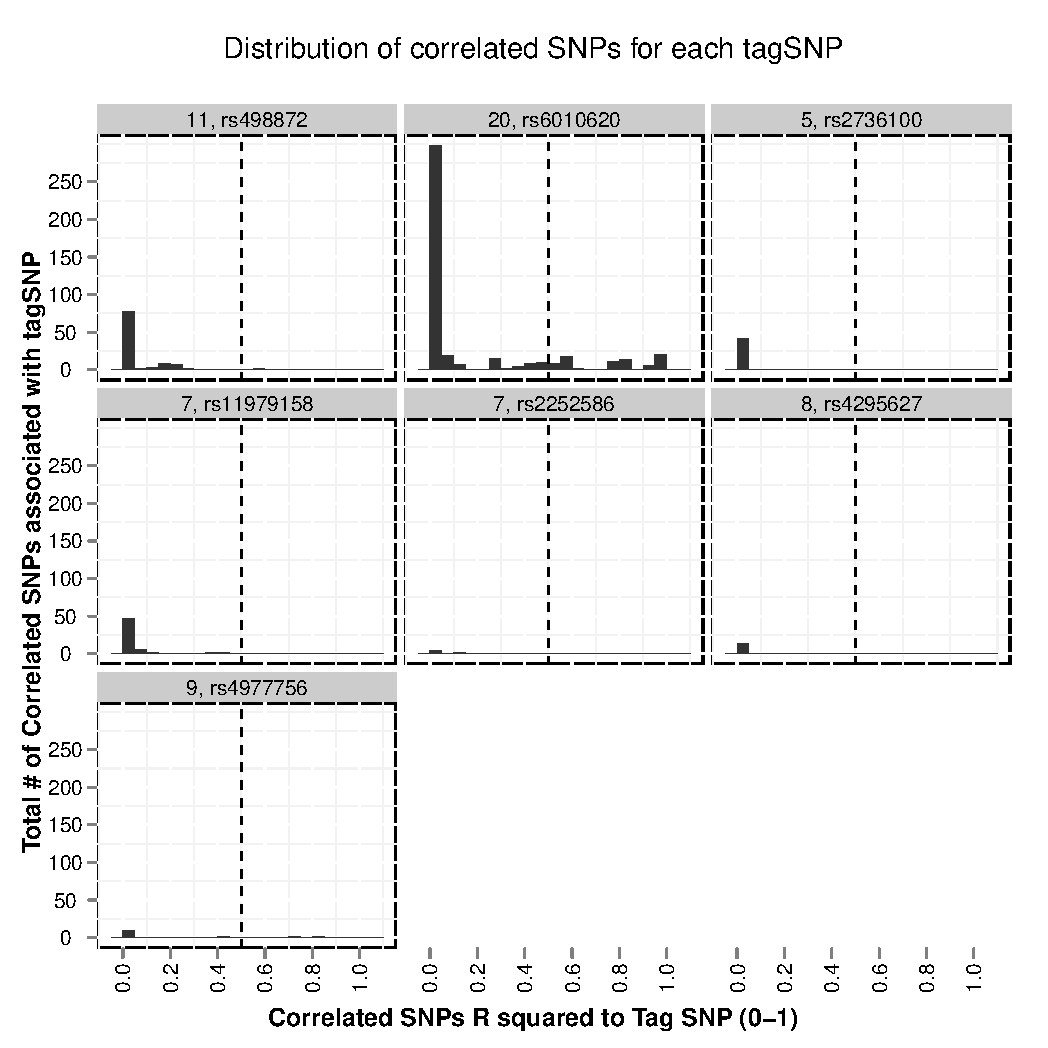
\includegraphics{glioma_dist_bysnp.pdf}
\caption{\label{fig:glioma_dist_bysnp.pdf} Distribution of Rsquare values of all
 Correlated SNPs divided by the tagSNP and it's location.}
{\footnotesize{}}
\end{center}
\end{figure}

\begin{Schunk}
\begin{Sinput}
> pdf("glioma_genomic_sum_rcut.pdf")
> FunciSNPplot(glioma.anno, rsq=0.5, genomicSum=T, save=F)
> dev.off()
\end{Sinput}
\begin{Soutput}
X11cairo 
       2 
\end{Soutput}
\end{Schunk}
\begin{figure}[ht!]
\begin{center}
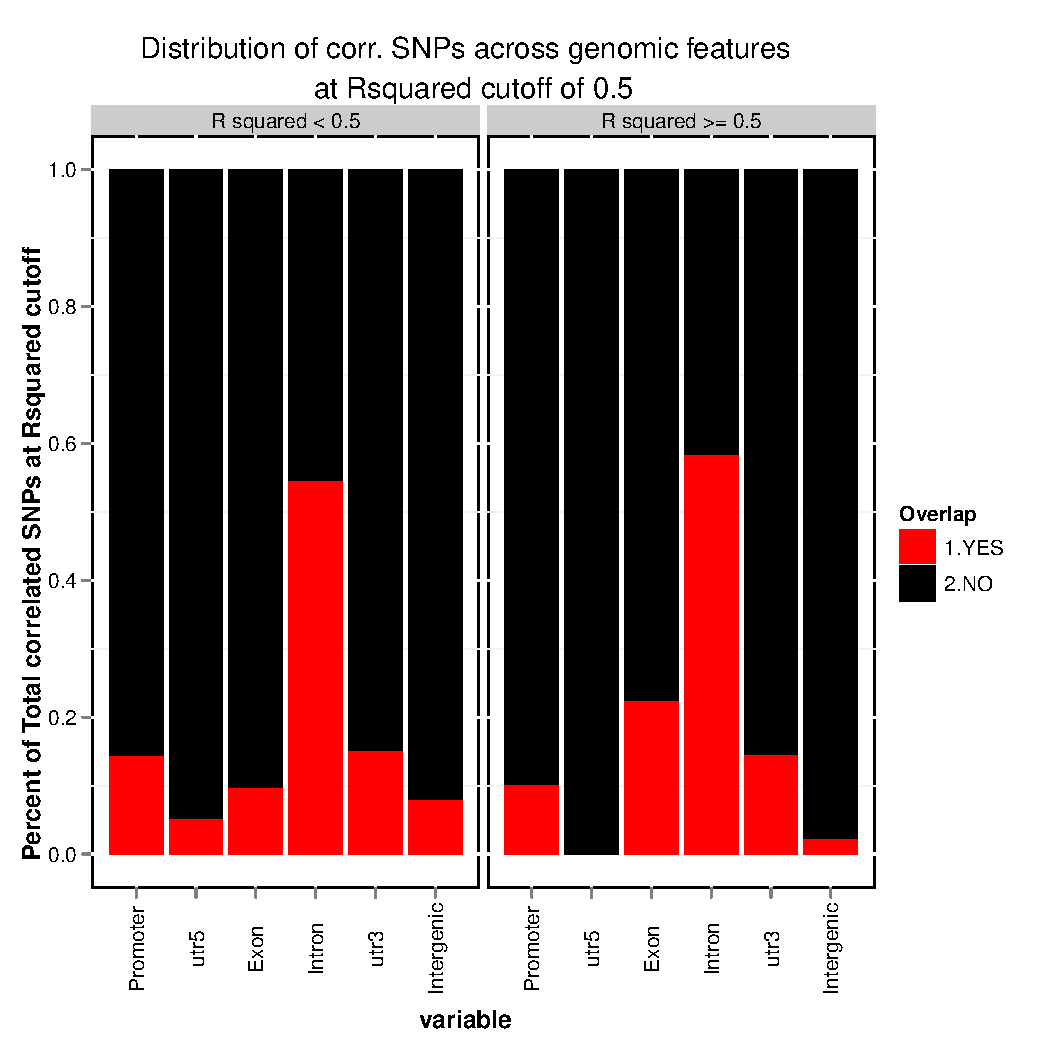
\includegraphics{glioma_genomic_sum_rcut.pdf}
\caption{\label{fig:glioma_genomic_sum_rcut.pdf} Stacked bar chart summarizing 
all correlated SNPs for each of the identified genomie features (exon, intron, 
5'UTR, 3'UTR, promoter, lincRNA or in gene desert (intergentic)). Rsquare cutoff
 at 0.5. This plot is most informative if used with a 'rsq' value.}
{\footnotesize{}}
\end{center}
\end{figure}

%<<>>=
%pdf("glioma_heatmap.pdf")
%FunciSNPplot(glioma.anno, rsq=0.5, heatmap=T, save=F)
%dev.off()
%@
%\begin{figure}[ht!]
%\begin{center}
%\includegraphics{glioma_heatmap.pdf}
%\caption{\label{fig:glioma_heatmap.pdf} Correlation heatmap to visualize the 
number of correlated SNPs at each tagSNP overlapping each biological feature. 
Rsquare cutoff at 0.5. This plot is most informative if used with a 'rsq' 
value.}
%{\footnotesize{}}
%\end{center}
%\end{figure}

Will output two plots per biofeature. The first plot is a scatter plot showing 
the relationship between Rsquare and Distance to tagSNP for each Func-y-SNP. The
 second plot is a histogram distribution of number of correlated SNPs at each 
 Rsquare value. Each set of plot is further divided by tagSNP. Best if used with
  'rsq' value.
\begin{Schunk}
\begin{Sinput}
> ## Following will output a series of plots for each biofeature at rsq=0.5
> FunciSNPplot(glioma.anno, tagSummary=T, rsq=0.5)
\end{Sinput}
\begin{Soutput}
Finished plotting  1 / 3 
Finished plotting  2 / 3 
Finished plotting  3 / 3 
\end{Soutput}
\end{Schunk}
\begin{figure}[ht!]
\begin{center}
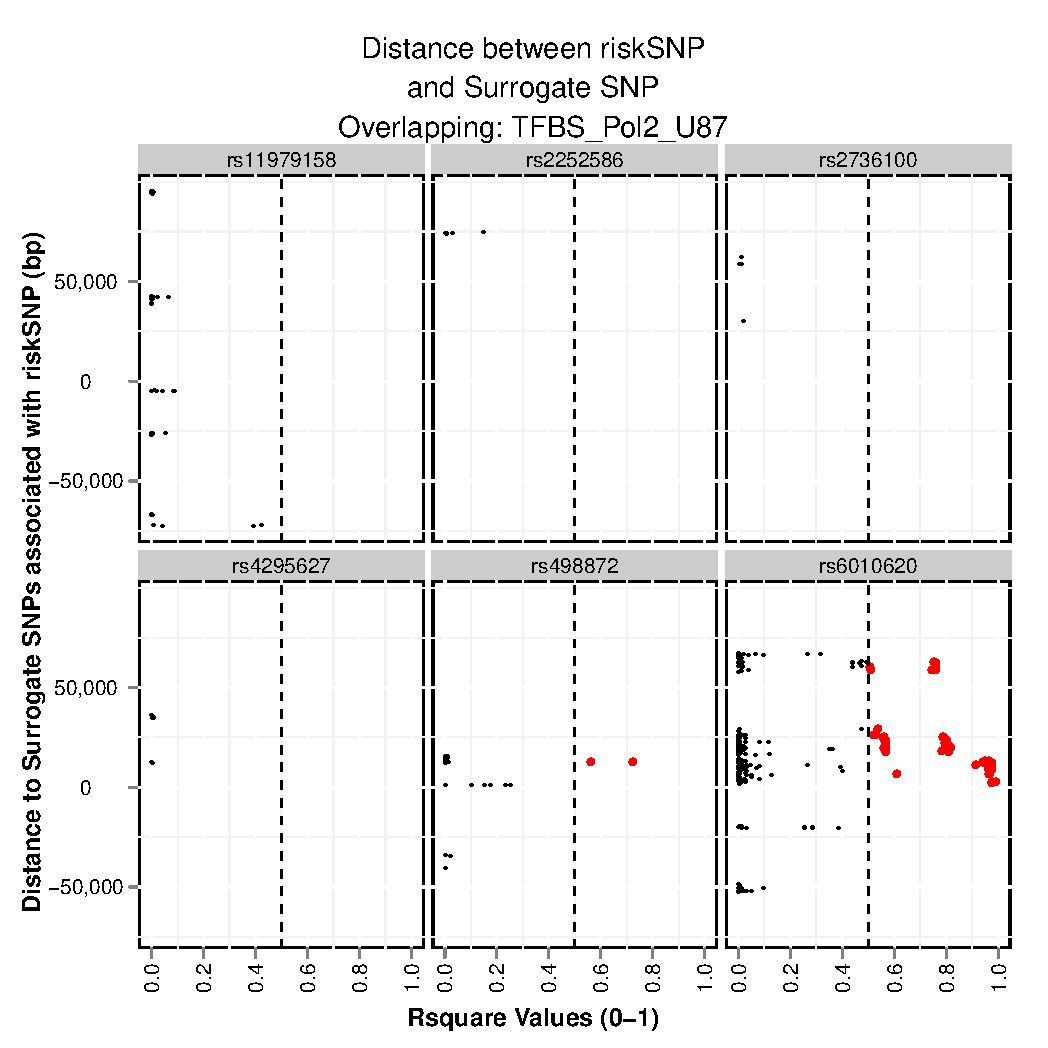
\includegraphics{FunciSNP.0.1.7/plots/TFBS_Pol2_U87_R2vsDist_riskSNP.pdf}
\caption{\label{fig:TFBS_Pol2_U87_R2vsDist_riskSNP.pdf} Scatter plot 
showing the relationship between Rsquare and Distance to tagSNP for each 
Func-y-SNP}
{\footnotesize{}}
\end{center}
\end{figure}

\begin{figure}[ht!]
\begin{center}
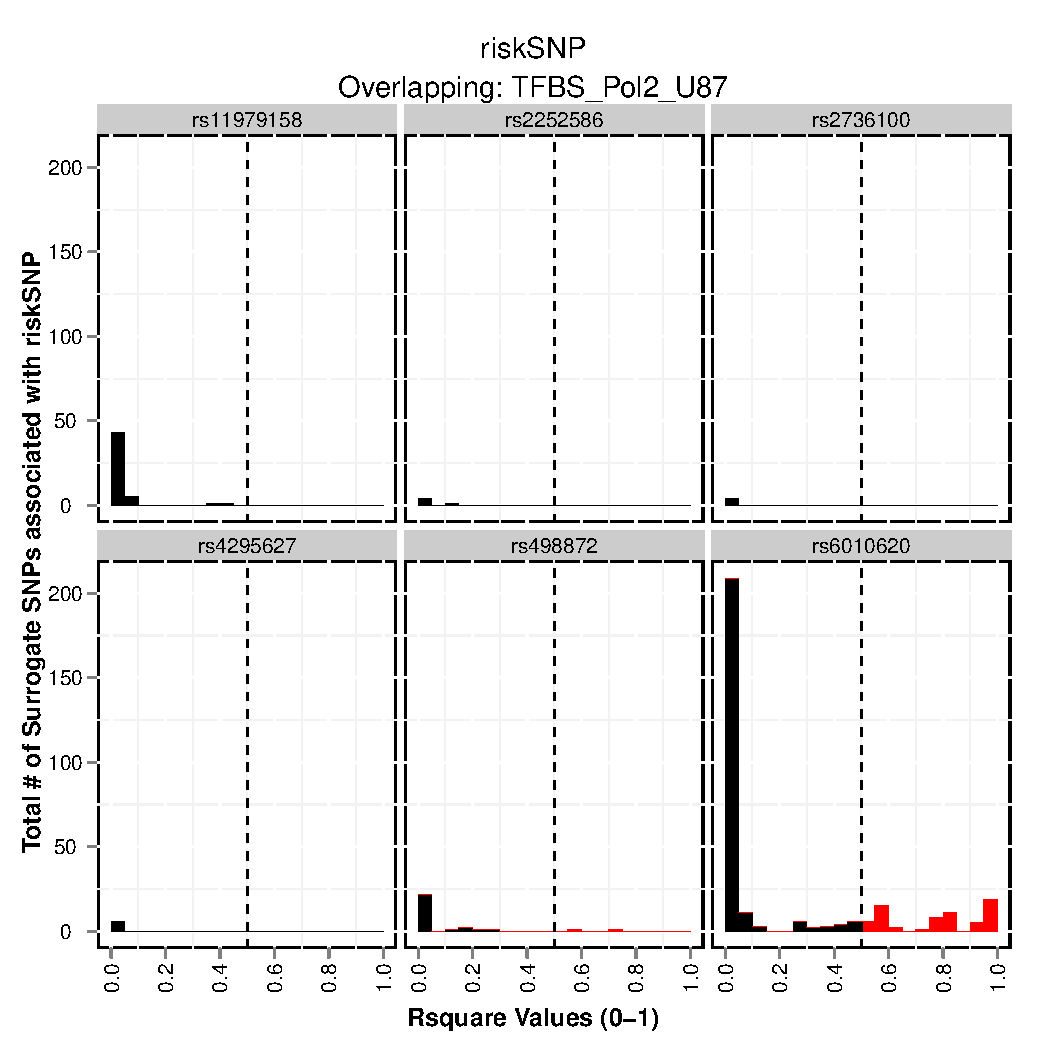
\includegraphics{FunciSNP.0.1.7/plots/TFBS_Pol2_U87_R2summary_riskSNP.pdf}
\caption{\label{fig:TFBS_Pol2_U87_R2summary_riskSNP.pdf} Histogram 
distribution of number of correlated SNPs at each Rsquare value}
{\footnotesize{}}
\end{center}
\end{figure}


\subsection*{FunciSNPbed()}
FunciSNPbed outputs a unique BED file which can be used to view in any genomic 
browser compatible with BED formats. To learn more about BED formats, see UCSC 
Genome Browser FAQ (http://genome.ucsc.edu/FAQ/FAQformat). Each tagSNP 
which is in LD to a corresponding Func-y-SNP overlapping at least one biofeature
 is colored black, while the Func-y-SNP is colored red. The initial position is 
 provided by the first tagSNP and the first linked Func-y-SNP. We recommend 
 using UCSC genome browser to view your BED files. This is useful so you can 
 view all public and private tracks in relation to FunciSNP results.
\begin{Schunk}
\begin{Sinput}
> ## will output to current working directory.
> FunciSNPbed(glioma.anno, rsq=0.5);
\end{Sinput}
\begin{Soutput}
Total corSNP (RED):  44 
Total tagSNP (BLK):  3 
\end{Soutput}
\end{Schunk}

\newpage

\begin{Schunk}
\begin{Sinput}
> sessionInfo()
\end{Sinput}
\begin{Soutput}
R version 2.14.1 (2011-12-22)
Platform: x86_64-pc-linux-gnu (64-bit)

locale:
 [1] LC_CTYPE=en_US.UTF-8       LC_NUMERIC=C              
 [3] LC_TIME=en_US.UTF-8        LC_COLLATE=en_US.UTF-8    
 [5] LC_MONETARY=en_US.UTF-8    LC_MESSAGES=en_US.UTF-8   
 [7] LC_PAPER=C                 LC_NAME=C                 
 [9] LC_ADDRESS=C               LC_TELEPHONE=C            
[11] LC_MEASUREMENT=en_US.UTF-8 LC_IDENTIFICATION=C       

attached base packages:
[1] stats     graphics  grDevices datasets  utils     grid      methods  
[8] base     

other attached packages:
 [1] FunciSNP_0.1.7        GenomicFeatures_1.6.7 GenomicRanges_1.6.4  
 [4] IRanges_1.12.5        matlab_0.8.9          gplots_2.10.1        
 [7] KernSmooth_2.23-7     caTools_1.12          bitops_1.0-4.1       
[10] gdata_2.8.2           gtools_2.6.2          org.Hs.eg.db_2.6.4   
[13] RSQLite_0.11.1        DBI_0.2-5             AnnotationDbi_1.16.11
[16] Biobase_2.14.0        BiocInstaller_1.2.1   ggplot2_0.8.9        
[19] proto_0.3-9.2         reshape_0.8.4         plyr_1.7.1           
[22] setwidth_0.9-4        colorout_0.9-9       

loaded via a namespace (and not attached):
 [1] annotate_1.32.1                        
 [2] biomaRt_2.10.0                         
 [3] Biostrings_2.22.0                      
 [4] bit_1.1-8                              
 [5] BSgenome_1.22.0                        
 [6] ChIPpeakAnno_2.2.0                     
 [7] digest_0.5.1                           
 [8] ff_2.2-4                               
 [9] genefilter_1.36.0                      
[10] GGBase_3.14.0                          
[11] GGtools_4.0.0                          
[12] GO.db_2.6.1                            
[13] lattice_0.20-0                         
[14] limma_3.10.2                           
[15] MASS_7.3-16                            
[16] Matrix_1.0-3                           
[17] multtest_2.10.0                        
[18] parallel_2.14.1                        
[19] RCurl_1.9-5                            
[20] Rsamtools_1.6.3                        
[21] rtracklayer_1.14.4                     
[22] snpStats_1.4.1                         
[23] splines_2.14.1                         
[24] survival_2.36-12                       
[25] tools_2.14.1                           
[26] TxDb.Hsapiens.UCSC.hg19.knownGene_2.6.2
[27] VariantAnnotation_1.0.5                
[28] XML_3.9-2                              
[29] xtable_1.6-0                           
[30] zlibbioc_1.0.0                         
\end{Soutput}
\end{Schunk}

\end{document}
